\newpage


\begin{figure}[t]
  \centering
  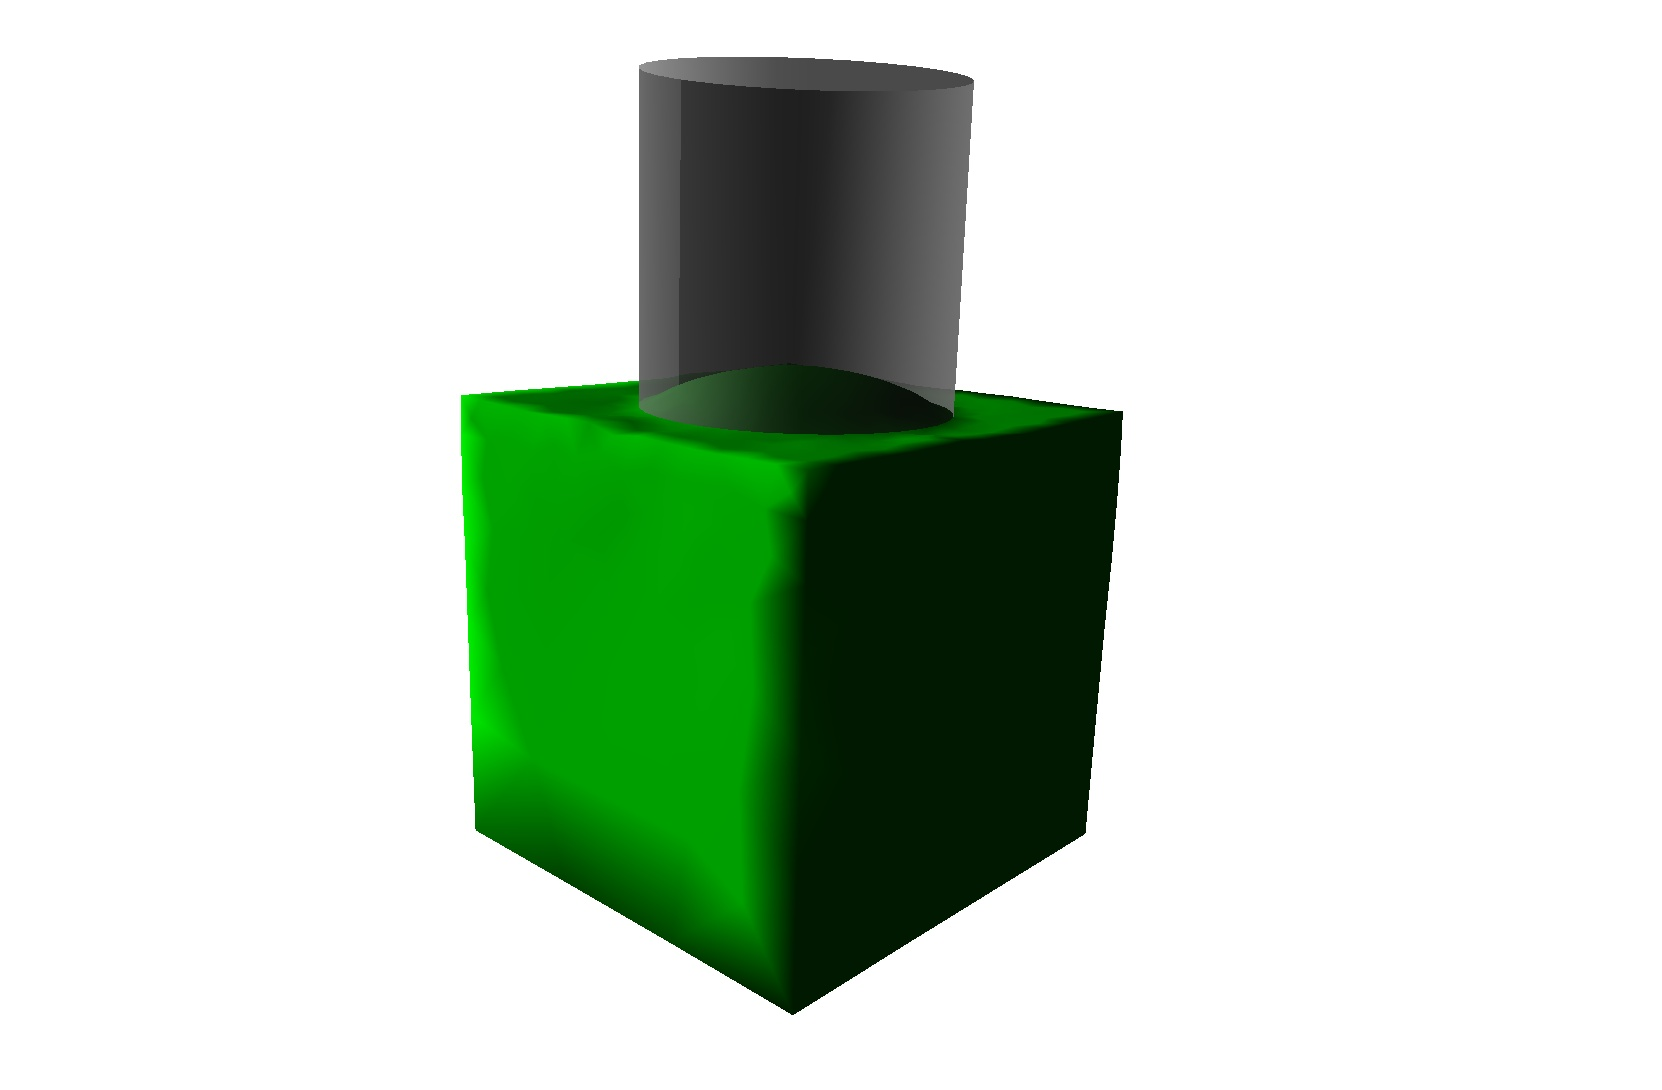
\includegraphics[height=3.5cm]{aspiration.jpg}
  \caption{\label{fig-aspiration1} The SOFA simulation scene of the aspiration test.}
\end{figure}

\begin{figure}[t]
  \centering
  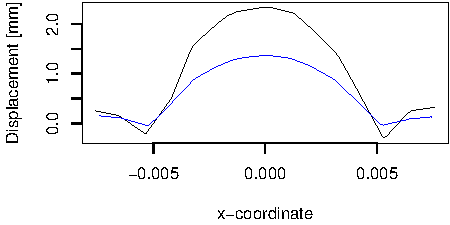
\includegraphics[width=7cm]{aspiration.pdf}
  \caption{\label{fig-aspiration2} Displacement profile of the cube in the
  aspiration test with (blue) and without (black) the capsule.}
\end{figure}

\begin{figure}
  \centering
  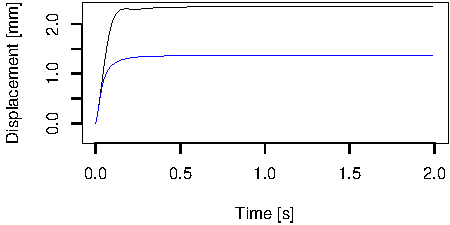
\includegraphics[height=3.5cm]{displacement.pdf}
  \caption{\label{fig-aspiration3} Evolution of the displacement at the center
  in time for test with (blue) and without (black) the capsule.}
\end{figure}

\begin{figure}[b]
  \centering
  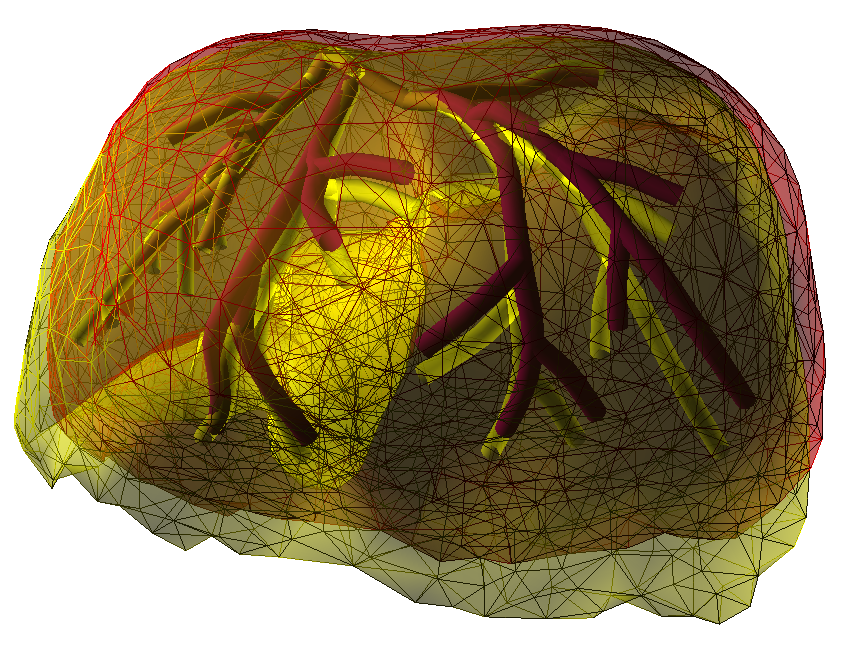
\includegraphics[height=7cm]{gravity2.png}
  \caption{\label{f:gravity} Liver under gravity with (red) and without (yellow) capsule}
\end{figure}
